\section{Thiết kế phần cứng}

\subsection{Nền tảng điều khiển}

Hệ thống sử dụng ESP32 NodeMCU-32S làm nền tảng điều khiển trung tâm. ESP32 được lựa
chọn vì tích hợp kết nối Wi-Fi, có nhiều giao tiếp ngoại vi như UART, ADC và GPIO, đồng
thời hỗ trợ tốt cho việc tổ chức firmware theo mô hình đa tác vụ. Với định hướng của đề
tài, ESP32 đóng vai trò nút biên thực hiện ba nhóm chức năng chính: thu thập dữ liệu từ
các cảm biến môi trường, xử lý và phản ứng cục bộ, đồng thời truyền dữ liệu lên backend
để phục vụ giám sát và điều khiển từ xa \cite{esp32soc}.

Trong cấu hình hiện tại, firmware sử dụng một UART cho cảm biến bụi PMS7003, một UART
khác cho bus RS485/Modbus và một kênh ADC cho cảm biến VOC dạng analog. Cách phân bố
này phù hợp với đặc tính tín hiệu của từng cảm biến, đồng thời tận dụng được các tài
nguyên phần cứng sẵn có trên ESP32 mà không cần thêm vi điều khiển phụ trợ.

\begin{figure}[H]
    \centering
    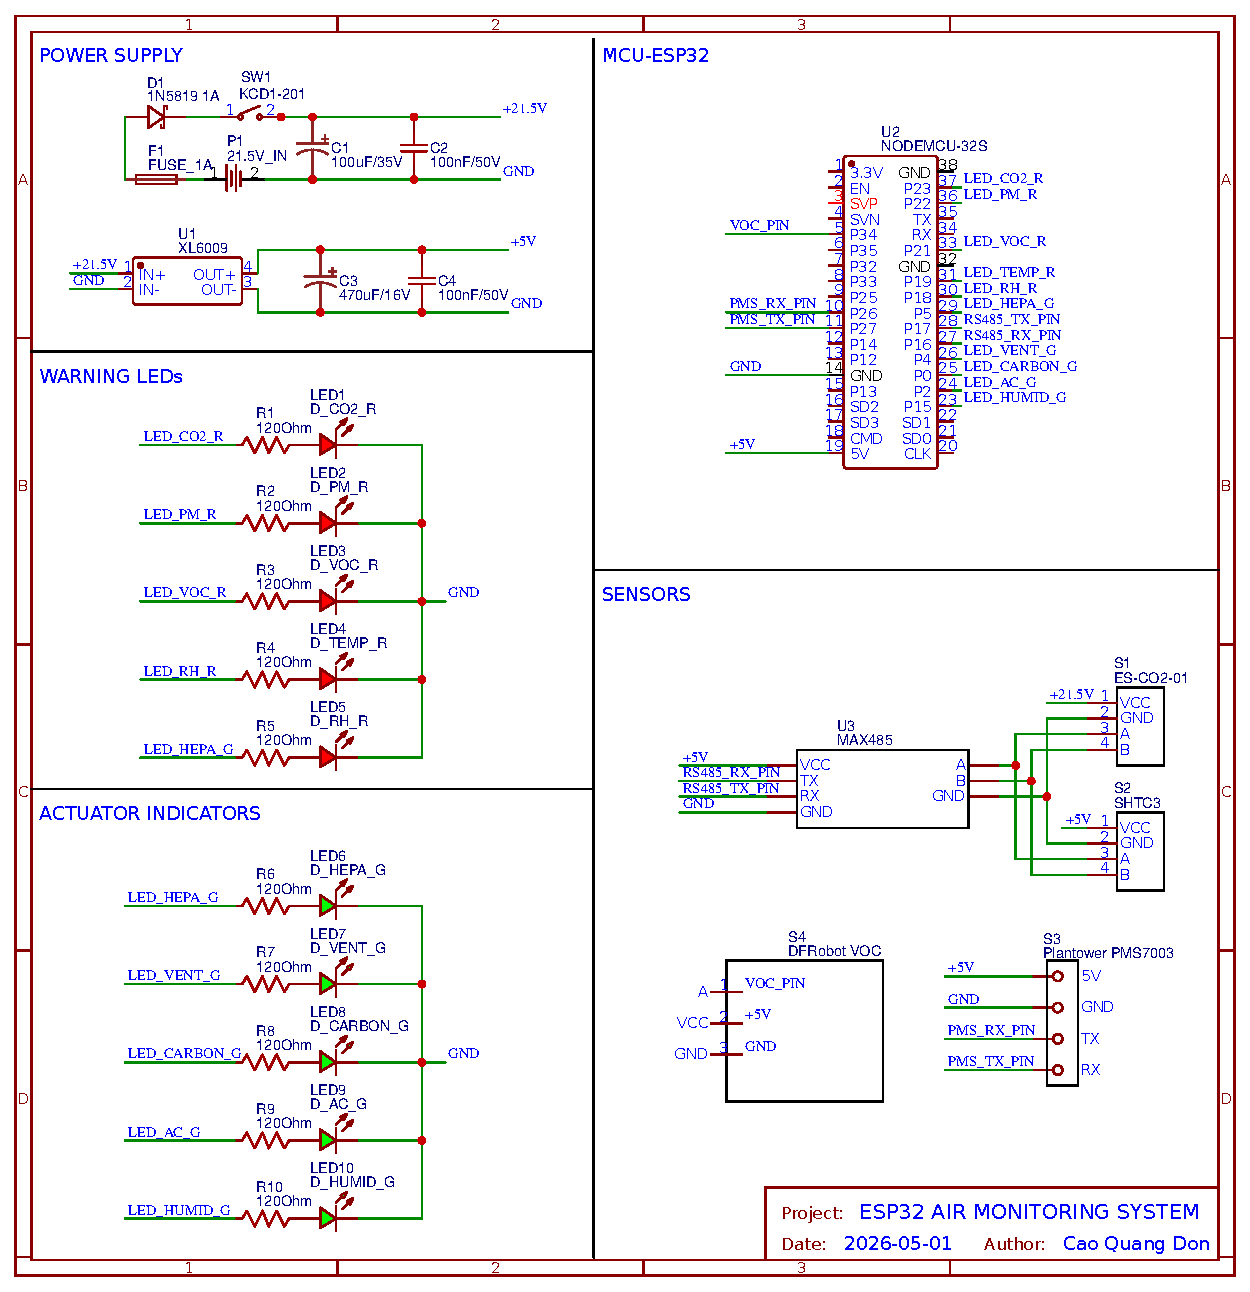
\includegraphics[width=\textwidth,page=1]{assets/Schematic_ESP32-Air-Monitoring-RS485-System_2026-05-16.pdf}
    \caption{Sơ đồ nguyên lý phần cứng của hệ thống}
    \label{fig:hardware-schematic}
\end{figure}

\begin{table}[H]
    \centering
    \caption{Pin map chính trong firmware}
    \begin{tabularx}{\textwidth}{>{\bfseries}l l X}
        \toprule
        Chức năng & Pin ESP32 & Ghi chú \\
        \midrule
        PMS RX & GPIO 26 & ESP32 nhận dữ liệu từ chân TX của PMS7003. \\
        PMS TX & GPIO 27 & Dự phòng khi cần gửi lệnh cấu hình cho PMS7003. \\
        RS485 RX & GPIO 16 & UART2 nhận dữ liệu phản hồi từ module RS485. \\
        RS485 TX & GPIO 17 & UART2 gửi request Modbus RTU đến các cảm biến RS485. \\
        RS485 DE/RE & \texttt{-1} & Source giả định module RS485 tự điều hướng truyền/nhận, firmware không điều khiển chân riêng. \\
        VOC ADC & GPIO 34 & Chân ADC1 input-only, dùng để đọc tín hiệu analog từ cảm biến VOC. \\
        \bottomrule
    \end{tabularx}
\end{table}

\subsection{Khối nguồn}

Hệ thống sử dụng nguồn một chiều đầu vào 21.5V làm nguồn cấp chính cho toàn mạch. Ở đầu
vào nguồn, cầu chì 1A được sử dụng để bảo vệ mạch khi xảy ra sự cố quá dòng hoặc chạm
chập. Diode Schottky 1N5819 được đặt nối tiếp nhằm bảo vệ mạch trong trường hợp đấu
ngược cực nguồn, đồng thời giảm tổn hao điện áp so với các diode chỉnh lưu thông thường.
Sau khối bảo vệ, nguồn được đưa qua công tắc ON/OFF để tạo nhánh nguồn đóng cắt chính
cho hệ thống.

Từ nhánh nguồn 21.5V sau công tắc, một hướng được cấp cho các cảm biến sử dụng mức áp
cao hơn, đồng thời một hướng được đưa vào bộ hạ áp LM2596 để tạo ra đường 5V cấp cho
ESP32 và các khối logic liên quan. Cách tổ chức này giúp tách rõ nhánh nguồn đầu vào và
nhánh nguồn hạ áp, đồng thời thuận lợi cho việc mở rộng phần cứng ở các phiên bản sau.

Tại nhánh 21.5V sau công tắc và tại đường 5V sau bộ hạ áp, mạch sử dụng kết hợp tụ
điện phân và tụ gốm mắc song song xuống mass. Tụ điện phân 100~$\mu$F ở phía đầu vào và
470~$\mu$F ở phía 5V đóng vai trò tụ đệm năng lượng, giúp giảm sụt áp tức thời khi tải
thay đổi. Tụ gốm 0.1~$\mu$F được dùng để triệt thành phần nhiễu cao tần trên đường
nguồn, từ đó cải thiện độ ổn định điện áp cấp cho vi điều khiển, module RS485 và các
cảm biến.

\subsection{Cảm biến và đặc tính kết nối}

Các cảm biến được lựa chọn nhằm theo dõi những đại lượng có ảnh hưởng trực tiếp đến chất
lượng không khí trong phòng học, bao gồm bụi mịn, CO\textsubscript{2}, nhiệt độ, độ ẩm
và VOC. Mỗi loại cảm biến sử dụng một phương thức giao tiếp phù hợp với đặc tính tín
hiệu và yêu cầu truyền dữ liệu.

Cảm biến bụi PMS7003 được dùng để đo các chỉ số PM1.0, PM2.5 và PM10. Cảm biến này làm
việc theo cơ chế xuất frame nhị phân qua UART ở tốc độ 9600 bps; trong firmware, driver
tìm cặp byte header \texttt{0x42 0x4D}, đọc đủ frame, kiểm tra checksum và sau đó tách
ra các giá trị bụi cần sử dụng \cite{pms7003}. Cách giao tiếp này đơn giản và phù hợp
với yêu cầu đọc dữ liệu bụi theo chu kỳ trên ESP32.

Cảm biến CO\textsubscript{2} và module nhiệt độ/độ ẩm được kết nối qua chuẩn RS485
Modbus RTU. Firmware tạo request với function code \texttt{0x03}, tính CRC16, gửi qua
UART2 và kiểm tra response trước khi cập nhật dữ liệu. Trong cấu hình hiện tại, cảm biến
CO\textsubscript{2} sử dụng slave ID 1 và đọc register \texttt{0x0001}; module nhiệt
độ/độ ẩm sử dụng slave ID 2 và đọc hai register bắt đầu từ \texttt{0x0000}. Việc sử
dụng RS485 giúp kết nối cảm biến theo hướng chống nhiễu tốt hơn và thuận lợi hơn cho mở
rộng bus cảm biến về sau \cite{modbus}.

Cảm biến VOC được đọc bằng ngõ vào ADC của ESP32. Do tín hiệu ở dạng analog và dễ dao
động theo nhiễu tức thời, lớp \texttt{VocAnalog} cấu hình attenuation cho ADC và sử
dụng bộ đệm vòng để tính trung bình trượt. Cách xử lý này giúp làm mượt dữ liệu trước
khi đưa vào tầng đánh giá IAQ, phù hợp với vai trò của VOC như một chỉ số xu hướng trong
nguyên mẫu hiện tại.

\subsection{Lý do lựa chọn giao tiếp cảm biến}

Việc lựa chọn giao tiếp cho từng cảm biến dựa trên đặc tính dữ liệu và mức độ ổn định
cần thiết của đường truyền. PMS7003 sử dụng UART vì cảm biến xuất dữ liệu dạng frame
liên tục, có header và checksum nên dễ kiểm tra tính hợp lệ. Đối với cảm biến
CO\textsubscript{2} và nhiệt độ/độ ẩm, RS485 Modbus RTU phù hợp hơn do hỗ trợ truyền
có dây ổn định, có địa chỉ slave và có CRC để phát hiện lỗi truyền. Trong khi đó, VOC
dùng ngõ vào ADC vì cảm biến xuất tín hiệu analog và không yêu cầu một giao thức truyền
số riêng.

Cách phân chia này giúp hệ thống tách rõ ba nhóm giao tiếp: UART frame cho cảm biến bụi,
Modbus register cho cảm biến RS485 và analog sampling cho cảm biến VOC. Nhờ đó, tầng
\texttt{SensorHub} có thể gom dữ liệu từ các nguồn khác nhau thành cùng một mẫu đo thống
nhất, trong khi các tầng xử lý phía sau không cần phụ thuộc trực tiếp vào chi tiết giao
thức của từng cảm biến.

\subsection{Thiết bị chấp hành và cảnh báo}

Trong phạm vi nguyên mẫu, hệ thống sử dụng LED để mô phỏng thiết bị chấp hành và cảnh
báo. Nhóm LED xanh biểu diễn trạng thái của các thiết bị hỗ trợ cải thiện chất lượng
không khí như thông gió, lọc HEPA, lọc than hoạt tính, điều hòa và tạo ẩm. Nhóm LED đỏ
biểu diễn cảnh báo theo từng nguyên nhân như CO\textsubscript{2}, bụi mịn, VOC, nhiệt
độ và độ ẩm.

Cách sử dụng LED giúp việc kiểm thử hệ thống trở nên trực quan hơn trong giai đoạn phát
triển mà không cần kết nối trực tiếp với các thiết bị công suất lớn. Khi một chỉ số môi
trường vượt ngưỡng, firmware có thể bật LED cảnh báo tương ứng; khi hệ thống phát lệnh
điều khiển thiết bị, LED xanh tương ứng sẽ thay đổi trạng thái để mô phỏng quá trình
bật hoặc tắt thiết bị. Mỗi LED được mắc nối tiếp với điện trở hạn dòng 120~$\Omega$ nhằm
giới hạn dòng qua LED, bảo vệ chân GPIO của ESP32 và duy trì độ sáng ở mức phù hợp cho
quan sát. Các chân điều khiển LED được khai báo trong \texttt{Pins.h} và có thể thay đổi
theo wiring thực tế.
